\chapter{Unsupervised Characterization of Water Composition with Generative Topographic Mapping}\label{ch:robot-team-gtm}

\textcolor{red}{Unmanned aerial vehicles equipped with hyperspectral imagers
  have emerged as an essential technology for the characterization of inland
  water bodies. The high spectral and spatial resolutions of these systems
  enable the retrieval of a plethora of optically active water quality
  parameters via band ratio algorithms and machine learning methods. However,
  fitting and validating these models requires access to sufficient quantities
  of in situ reference data which are time-consuming and expensive to obtain. In
  this study, we demonstrate how Generative Topographic Mapping (GTM), a
  probabilistic realization of the self-organizing map, can be used to visualize
  high-dimensional hyperspectral imagery and extract spectral signatures
  corresponding to unique endmembers present in the water.  Using data collected
  across a North Texas pond, we first apply  GTM to visualize the distribution
  of captured reflectance spectra, revealing the small-scale spatial variability
  of the water composition. Next, we demonstrate how the nodes of the fitted GTM
  can be interpreted as unique spectral endmembers. Using extracted endmembers
  together with the normalized spectral similarity score, we are able to
  efficiently map the abundance of nearshore algae, as well as the evolution of
  a rhodamine tracer dye used to simulate water contamination by a localized
  source. }



\section{Motivation}

Inland water bodies present a unique challenge to characterization by remote sensing imagery due to their complex spectral characteristics and small-scale spatial variability. The broad bands of multispectral imagers coupled with the irregular shape of lakes and rivers result in pixels with highly mixed signals that are easily dominated by reflectance from shore and nearshore vegetation sources \cite{koponen2002lake, ritchie2003remote}. Recently, the combination of hyperspectral imaging with unmanned aerial vehicles (UAVs), such as drones, has emerged as a powerful approach to simultaneously address the spectral, spatial, and temporal limitations of traditional high-altitude and satellite-based collection \cite{adao2017hyperspectral,arroyo2019implementation}. UAVs are significantly less expensive to deploy than their satellite- or aircraft-based remote sensing counterparts, and low-altitude flights enable centimeter-scale sampling while limiting the need for complicated atmospheric corrections \cite{banerjee2020uav}. However, the significant increase in the data volume generated by these systems presents a new challenge, namely, how to efficiently extract water quality parameters of interest from intricate pixel spectra.

Significant research efforts have focused on the development of techniques and algorithms to retrieve water quality parameters from UAV-captured hyperspectral images (HSI). Onboard computers installed alongside hyperspectral imagers enable the rapid evaluation of spectral indices from HSI band ratios \cite{horstrand2019uav}. These band ratios and polynomial combinations of bands have been used to successfully invert optically active water quality parameters such as turbidity directly from UAV-acquired imagery \cite{vogt2016near, zhang2022selection}. Supervised machine learning techniques such as tree-based models, support vector machines, and neural networks have also been used to estimate a wide range of parameters, such as colored dissolved organic matter, chlorophyll A, blue--green algae, and suspended sediment concentrations \cite{keller2018hyperspectral, lu2021retrieval}. % Please check intended meaning is retained.
The calibration and evaluation of these data-driven models require a significant volume of coincident in situ data. This can be streamlined by coordinating UAV flights with reference data collection using autonomous robotic boats \cite{robot-team-1, robot-team-2}. New proximal sensors for water quality parameters are continually being developed \cite{proximal-sensing-1, proximal-sensing-2}. However, this approach relies on the prior knowledge of expected sources in order to select appropriate reference instruments for model validation. The presence of unanticipated contaminants cannot be directly identified in this sensing paradigm.

Extending the capabilities of UAV-based hyperspectral imaging to enable water quality monitoring in real-time scenarios where contaminant sources may not be known in advance requires two additional capabilities: dimensionality reduction techniques to permit the visual comparison of HSI and endmember extraction techniques which can identify spectral signatures corresponding to unique sources within the imaging scene. In remote sensing where reference data are typically sparse, many approaches have been explored. For example, principal component analysis (PCA) and t-distributed stochastic neighbor embedding (tSNE) are dimensionality reduction methods commonly used to reduce HSI to two or three dimensions for visualization \cite{tyo2003principal,zhang2015hyperspectral}. Similarly for endmember extraction, there are a variety of established approaches including geometric methods like vertex component analysis, statistical methods like k-nearest neighbors and non-negative matrix factorization (NMF), and deep learning methods based on autoencoder architectures \cite{heylen2014review,vca-orig, unmixing-nmf-review-2, cariou2015unsupervised, su2019daen, borsoi2019deep, palsson2020convolutional}. Methods based on linear mappings like PCA and NMF are often too restrictive for HSI, where the assumption of linear mixing is easily broken. However, the increased complexity of nonlinear methods like tSNE and autoencoders often lead to significant increases in computation time. An ideal approach should enable both visualization and nonlinear identification of relevant spectral endmembers.

% neurons that wire together, fire together
The self-organizing map (SOM) developed by Teuvo Kohonen is an unsupervised machine learning method which nonlinearly maps high-dimensional data to the nodes of a two-dimensional grid \cite{kohonen-som-1}. By preserving the topological relationship between nodes during training, the SOM ensures that similar spectral signatures are mapped together such that related HSI pixels naturally cluster together. This presents an attractive compromise by enabling the simultaneous visualization of HSI data and endmember extraction via the weight vector associated with each SOM node \cite{cantero2004analysis, duran2007time,som-hsi}. When reference data are available, the SOM can be utilized to provide semisupervised labeling of HSI spectra~\cite{riese2019supervised}. Furthermore, Danielsen et al. demonstrated that the dimensionality reduction offered by the SOM can even be used for onboard data compression of HSIs acquired by a CubeSat \cite{danielsen2021self}. Despite these clear capabilities, the SOM relies on a heuristic training algorithm with hyperparameters that can be challenging to tune and offers no direct probabilistic interpretation. To address these limitations, Bishop et al. developed  generative topographic mapping (GTM), a probabilistic latent-variable model inspired by the SOM \cite{gtm-orig}.  GTM has been utilized in a variety of domains, including drug design and chemical data visualization, but has yet to see adoption for the analysis of hyperspectral imagery \cite{kireeva2012generative, gaspar2015chemical, horvath2019generative}.

In this study, we explore the application of  GTM to UAV-acquired HSI for the characterization water quality. Using data collected at a pond in Montague, North Texas, we first train a GTM using water-only pixels to produce a low-dimensional representation of the collected HSI. We use this mapping to explore the highly detailed small-scale variability within the pond and discuss how this can be used to guide reference data collection. Next, we demonstrate how  GTM can be utilized to identify relevant spectral endmembers from a combined dataset including ground pixels, nearshore filamentous blue--green algae, water, and a simulated contaminant plume using a rhodamine tracer dye. Once identified, these endmembers can be used to rapidly map the abundance of spectral features within the pond. We demonstrate this capability by using  GTM to map the abundance of filamentous blue--green algae near the shore, as well as the dispersion of a rhodamine dye plume.


\section{Unsupervised Learning}

\subsection{Self Organizing Maps}

Self organizing maps (SOMs) are an unsupervised machine learning technique developed by Kohonen \cite{kohonen-original} based on the simple biological principle that \textit{neurons near each other fire together}. This observation that the toplogical \textit{closeness} of similar computational units is a critical feature of intelligent systems leads to a natural reinterpretation of the familiar perceptron model into a new form amenable for a variety of clustering and dimensionality reduction tasks. In particular, the SOM enables a rapid unsupervised classification of multidimensional data into a (typically) one or two dimensional \textit{simplicial complex}, the discrete realization of a topological manifold, whose vertices correspond to representative points in the original data space $\mathcal{D}$. While a tad esoteric compared to other popular unsupervised methods like KMeans clustering or DBSCAN, the SOM distinguishes itself with the added benefit that it's training procedure guarantees nodes (i.e. classes) close to each other in the feature manifold share similar weights. This additional structure makes the SOM particularly attractive when an interpretation of the discovered clusters as well as the relationships between them is desired.

The original treatment of the SOM by Kohonen was made in terms of processing units, sensory signals, and relaying networks \cite{kohonen-original}, however, in the modern era of deep learning, a more easily digestible derivation can be obtained by re-interpreting the weights of a simple perceptron model to provide the foundation for a clustering approach. As described in previously, a perceptron is a function of the form
\begin{equation}
    \mathbf{y} = \sigma.\left(W\mathbf{x}\right)
\end{equation}
where $W\in\mathbb{R}^{n\times m}$ is a matrix of weights which transform the input $\mathbf{x}\in\mathbb{R}^m$ into $\mathbb{R}^n$ and $\sigma$ is a nonlinear \textit{activation function} applied element-wise to the outputs of the matrix multiplication (indicated by the $.$ syntax). If we instead think of the weight matrix as an ordered collection of vectors $\{\mathbf{w}_i\}_{i=1}^{n}$, then this formula can be further decomposed into
\begin{equation}
    (\mathbf{y})_i = \sigma(\mathbf{w}_i^T\mathbf{x}) = \sigma(\langle \mathbf{w}_i, \mathbf{x} \rangle)
\end{equation}
The function of the perceptron is now clear: given an input vector $\mathbf{x}$ and a collection of $n$-many weight vectors $\mathbf{w}_i$, compute the $n$-many inner products of $\mathbf{x}$ with each weight vector $\mathbf{w}_i$, apply the nonlinear activation function $\sigma$, and concatenate the results.

If we now allow ourselves to imagine the weight vectors $\mathbf{w}_i$ as members of the same vector space as the input $\mathbf{x}$, a reasonable question to ask is: \textit{how similar is the input $\mathbf{x}$ to each $\mathbf{w}_i$}. Further, the application of the inner product $\langle \cdot,\cdot \rangle$ suggests we may answer this question in terms of the distance
\begin{equation}
    \langle \mathbf{w}_i-\mathbf{x},  \mathbf{w}_i-\mathbf{x}\rangle = d(\mathbf{w}_i, \mathbf{x})^2.
\end{equation}
In other words, given a set of weight vectors $\mathbf{w}_i$ which we may now think of as the cluster centers for our unsupervised model, we can measure the similarity between a given datum $\mathbf{x}_j$ and each cluster by computing the distance
\begin{equation}
    d_{ij} = d\left(\mathbf{w}_i, \mathbf{x}_j \right).
\end{equation}

To make this mapping useful, we should prescribe a \textit{training procedure} which updates the vectors $\mathbf{w}_i$ based on all of the available data points. Further, our goal is to establish some kind of interpretable relationship between the various weights $\mathbf{w}_i$ so that they \textit{more than} disjoint classes. The SOM achieves this by providing a lower-dimensional grid (typically 2-dimensional) whose vertices are understood to be the location of each of the weight vectors. The procedure is as follows:

First, initialize a grid of weight vectors $\mathbf{w}_i\in\R^m$ which we collect into a matrix $W\in\R^{m\times n}$. Assign coordinates to each weight vector by mapping each $\mathbf{w}_i$ to a vertex in the grid. The \textit{topology} of the grid is a hyperparameter which dictates the spatial relationship between neighboring nodes. Popular choices are: flat rectangular, rectangular on a cylinder (one periodic boundary condition), rectangular on a torus (two periodic boundary conditions), hexagonal (more equidistant neighbors per node than rectangular), and spherical.
\begin{figure}[h]
  \centering
  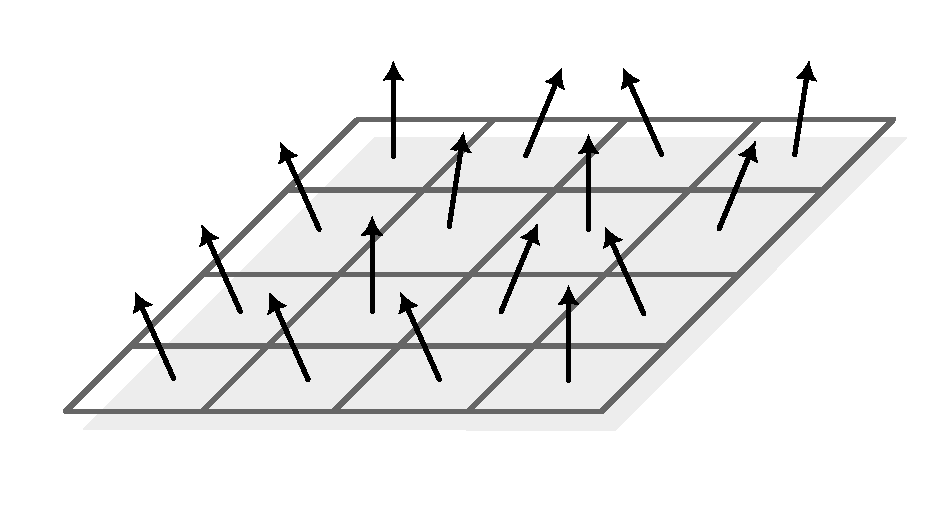
\includegraphics[width=0.75\columnwidth]{robot-team-gtm/som/som-diagram.pdf}
  \caption{A Self Organizing Map with nodes configured in a rectangular grid topology with weight vectors randomly initialized.}
  \label{fig:som-diagram}
\end{figure}
One can initialize the weights in a variety of ways. Some common choices are
\begin{itemize}
\item Randomly initialize them as in figure \ref{fig:som-diagram}.
\item Initialize them to the value of $n$-many randomly selected data samples $\mathbf{x}_i$.
\item Initilize them to the first $n$-many principal components of the dataset.
\end{itemize}

Next, we proceed to update the weights according to the following steps for each $\mathbf{x}_k$ datum:
\begin{enumerate}
\item Compute the \textit{best match unit} (BMU) as
  \begin{equation}
    \mathbf{w}_{i}^{\text{best}} = \text{arg}\min\limits_{\mathbf{w}_j} \left( d(\mathbf{x}_k, \mathbf{w}_j)^2 \right)
  \end{equation}
  where $d(\cdot,\cdot)$ is some suitably chosen distance function. One often defaults to the Euclidean metric.
\item Choose a radius $\sigma_t$ which we will use to identify the correct update for to apply to all nodes relative to $\mathbf{w}_i^{\text{best}}$.
\item Update \textit{all} the weights according to the equation
  \begin{equation}
    w_{m}^{t+1} = w_m^{t} + \eta(t)f(x_m,y_n,\sigma_t)\left(\mathbf{x}_k  - \mathbf{w}_n^{t} \right)
  \end{equation}
  where $\eta(t)$ is the learning rate, and $f(x_m, y_m, \sigma_t)$ is the \textit{neighborhood} function which defines the relative amount each node $\mathbf{w}_m$ is updated according to its coordinate distance from the best match unit (i.e. the distance between the points $(x_m, y_m)$ and $(x_{\text{best}}, y_{\text{best}})$ in the two dimensional case). Typically one chooses a the learning rate to evolve according to the schedule
  \begin{equation}
    \eta(t) = \eta_0\exp(^-\lambda t)
  \end{equation}
  with the radius $\sigma_t$ evolving similarly according to
  \begin{equation}
    \sigma_t = \sigma_0\exp(-\beta t).
  \end{equation}
  Popular choices for the neighborhood function are the Gaussian function, Mexican-hat function, a cone function, and a cylinder function.
\end{enumerate}


As an illustrative example, consider the minimal dataset formed by the colors red, green, and blue which as vectors may be written as
\begin{align}
  \text{Red} &= \left(1,\; 0,\; 0 \right)\\
  \text{Green} &= \left(0,\; 1,\; 0 \right) \\
  \text{Blue} &= \left(0,\; 0,\; 1 \right).
\end{align}
Now let us suppose we want to train an SOM to generate a classification for colors using only these three as the supplied training data. Figure \ref{fig:som-demo} shows exactly this. Here we have trained an SOM of size $25 \times 25$ cells in a flat hexagonal topology. As the weight vectors are themselves vectors of length $3$, we can then visualize the trained SOM by coloring each corresponding node by the color learned in its weight vector. What we find is that the resulting map has clearly separated red, green, and blue into distinct regions in the grid, and more importantly, there is a smooth gradient between neighboring cells reflecting the fact that neighboring classes are more \textit{similar} than cells with a large separation distance. This is not the case for many other common clustering techniques like k-nearest neighbors or DBSCAN for which relationship between learned classes is challenging to interpret.

\begin{figure}[h!]
  \centering
  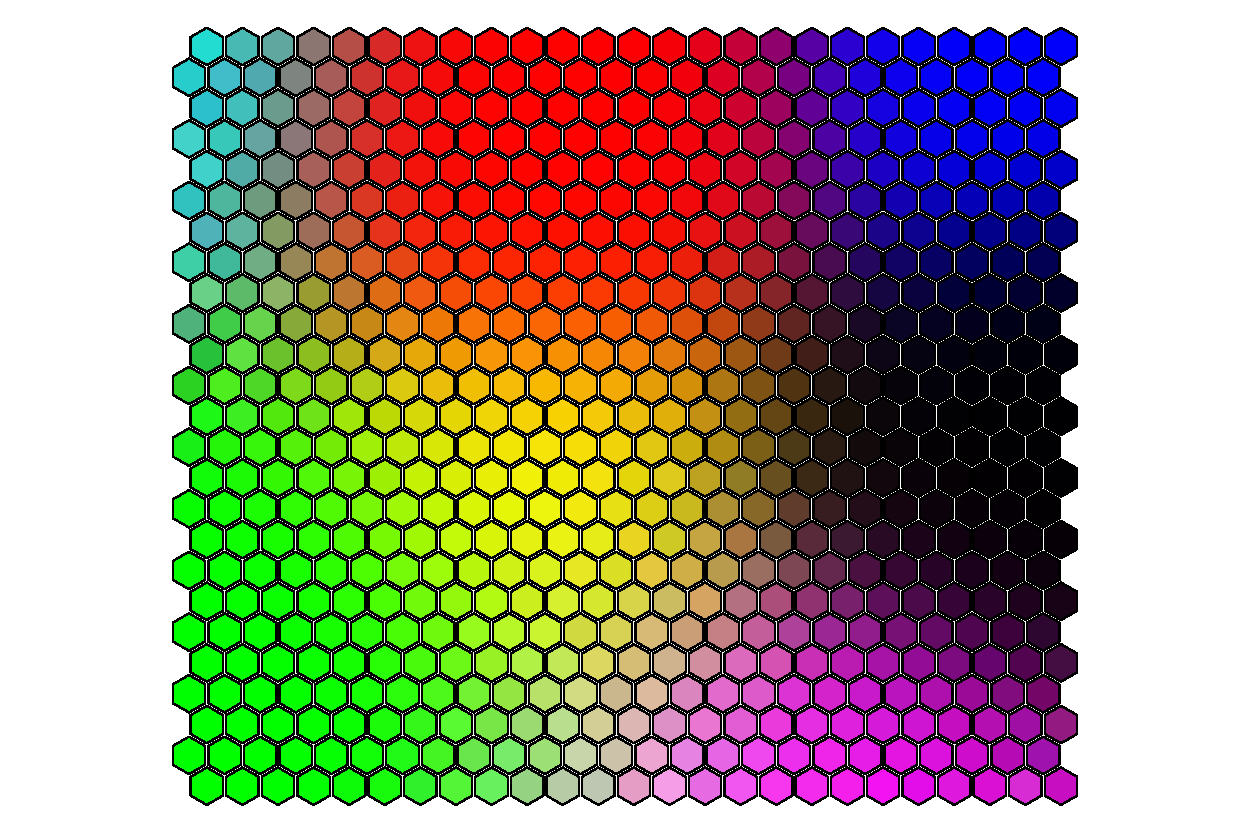
\includegraphics[width=0.75\columnwidth]{robot-team-gtm/som/SOM_demo.pdf}
  \caption{A trained Self Organizing Map of $25\times 25$ cells in a hexagonal topology trained on a dataset consisting of the three colors red, green, and blue.}
  \label{fig:som-demo}
\end{figure}

To enable this demonstration and its subsequent use throughout the rest of this dissertation, I have created a new open-source implementation of the SOM algorithm for the Julia programming language called \texttt{SelfOrganizingMaps.jl} which has been added to the general registry and can by freely downloaded for use by anyone. The repository for the code as well as the associated documentation can be found at \href{https://github.com/john-waczak/SelfOrganizingMaps.jl}{this site}.


\subsection{Expectation Maximization}

\subsection{Generative Topographic Mapping}


\section{Study Overview}


In this study, we explore the use of  GTM as a tool for dimensionality reduction
and unsupervised endmember extraction of hyperspectral imagery. To this end, a
dataset of HSI was collected at a pond in Montague, North Texas, on 23 November
2020 using a UAV-mounted hyperspectral imager configured as described in
\cite{robot-team-1, robot-team-2}. The pond spans an area $<0.1$ $\text{km}^2$
and has a maximum depth of $3$ m. Across multiple flights, many data cubes like
the example shown in panel a of Figure~\ref{fig:sample-spectra} were collected.
Additionally, rhodamine dye was released and subsequently imaged to simulate a
localized contaminant source. Using the HSI shown in
Figure~\ref{fig:sample-spectra}, a set of exemplar spectra were visually
identified corresponding to nearshore filamentous blue--green algae, water,
rhodamine dye, and the ground (a combination of soil and dry grass). The
location of these samples is shown in panel b and their corresponding
reflectance spectra are visualized in panel c.  In the remainder of this
section, we first provide a detailed overview of the GTM algorithm. Next, we
describe the UAV platform used for HSI collection and the various steps employed
to process captured HSI. Finally, we describe the two case studies presented in
this paper for the utilization of  GTM as an HSI visualization tool and as an
endmember extraction technique.



\begin{figure}[H]
  \centering
  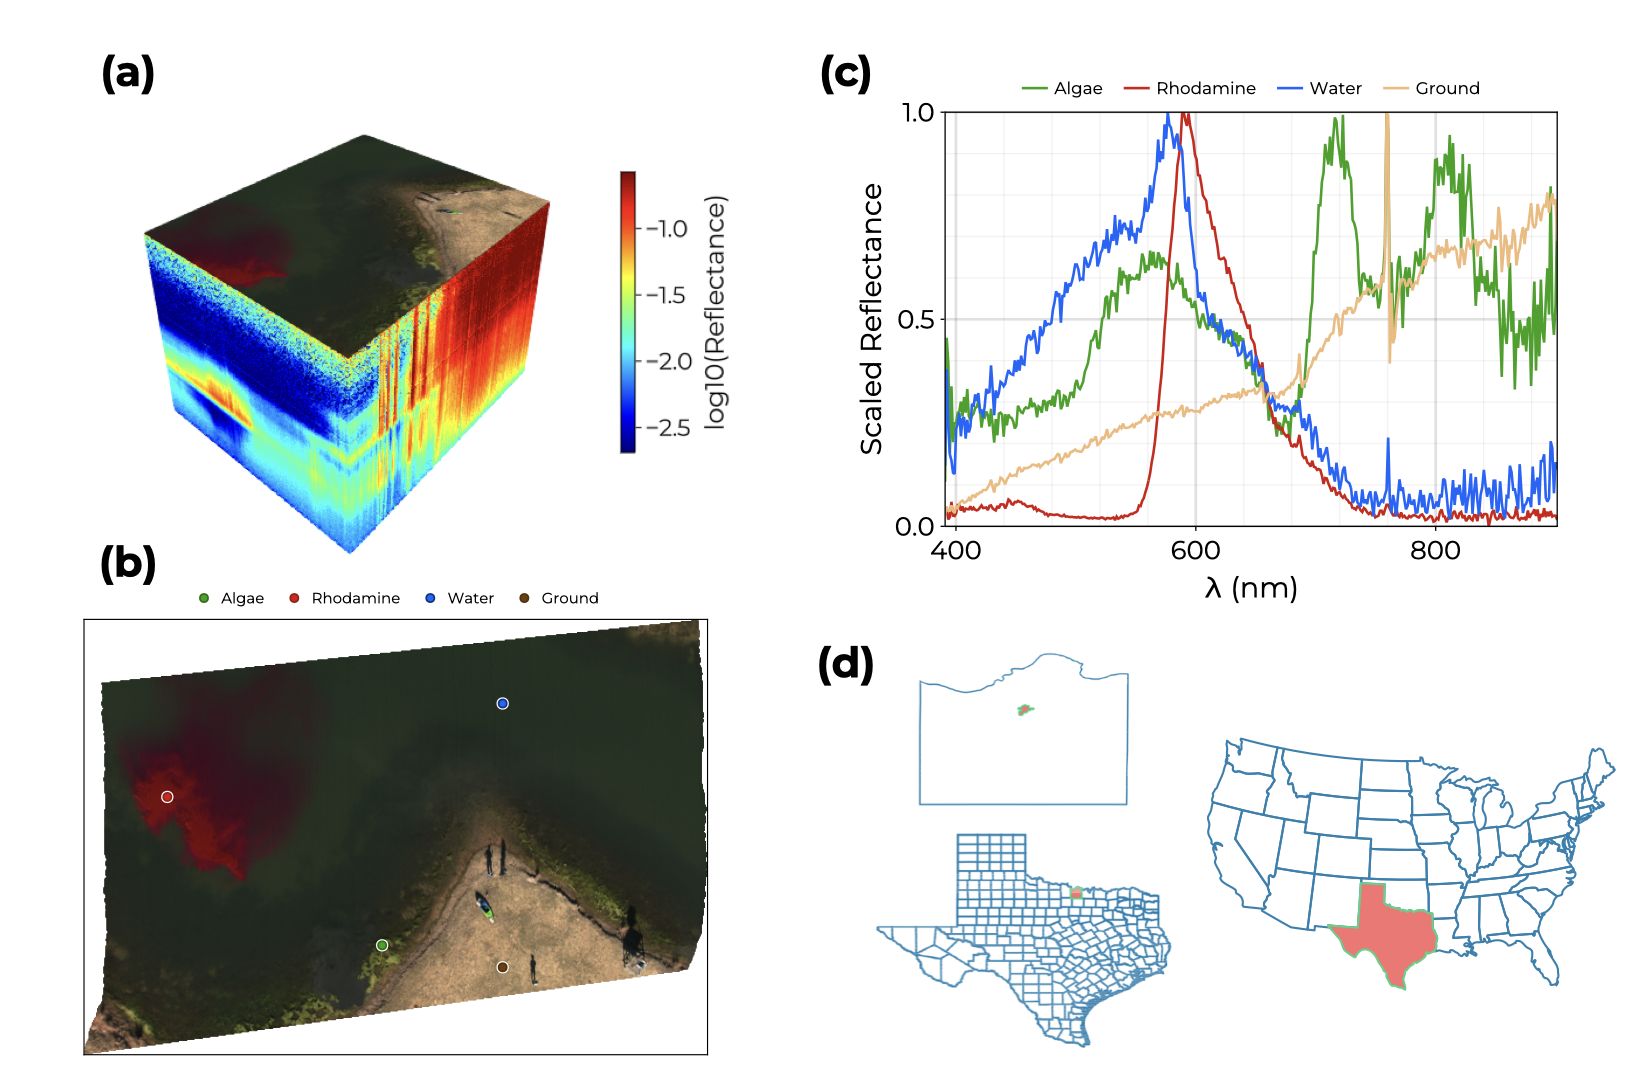
\includegraphics[width=\columnwidth]{robot-team-gtm/methods/sample-spectra.png}
  \caption{(\textbf{a}) Sample hyperspectral data cube. Spectra are plotted
    using their geographic position with the log10-reflectance colored along the
    \emph{z} axis and a pseudocolor image on top. (\textbf{b}) Points taken from
    a sample hyperspectral data cube corresponding to algae, rhodamine dye,
    water, and ground (dirt and dry grass). (\textbf{c}) Reflectance spectra for
    the exemplar points scaled so the peak value of each spectrum is $1.0$.
    (\textbf{d}) The location of the pond in Montague, Texas, where data were
    collected for this study.}
    \label{fig:sample-spectra}
\end{figure}

%%% --- Generative Topographic Mapping ------------------------------------
\subsection{Generative Topographic Mapping}\label{sec:gtm-overview}

GTM is a probabilistic latent-variable model inspired by the  SOM for visualizing and clustering high-dimensional data. Like the  SOM, GTM assumes vectors $\mathbf{x}$ in the $d$-dimensional data space (here representing reflectance spectra) are constrained to a low-dimensional embedded manifold. The SOM describes this manifold using a regular grid of nodes, each having an associated weight vector defining the mapping from the manifold to the data space. The position of each data record $\mathbf{x}$ in the manifold is assigned to the position of the node whose weight vector has the minimum Euclidean distance to $\mathbf{x}$. An iterative training procedure updates the weight vectors of each node to fit the manifold to the data such that nodes near each other in the SOM grid correspond to similar records in the data space.

GTM mimics the grid of the SOM by assuming data are generated from latent variables $\xi$ that are constrained to the $K$-many nodes of a regular grid. This assumption corresponds to establishing a prior distribution on the latent space of the form
\begin{equation}\label{eq:latent-prob}
    p(\xi) = \frac{1}{K}\sum_k^K \delta(\xi - \xi_k)
\end{equation}
where $\delta(\cdot)$ is the Dirac delta function.

Points $\xi$ in this latent space are mapped to the embedded manifold by a nonlinear function $\psi$ parameterized by weights $W$. However, since real data are rarely noise-free, this embedded manifold will not be perfectly thin. To account for this, the points $\xi$ are described in the data space by a radially symmetric Gaussian distribution, $\mathcal{N}(\psi(\xi),\, \beta^{-1})$, with mean $\psi(\xi)$ and precision $\beta$. For a dataset $\left\{ \mathbf{x}_n\right\}_{n=1}^N$ consisting of $N$-many records, this choice yields a log-likelihood function of the form
\begin{equation}\label{eq:llh}
    \mathcal{L}(W, \beta) = \sum_n^N \ln \left(\dfrac{1}{K}\sum_k^K p(\mathbf{x}_n \mid \xi_k, W, \beta) \right)
\end{equation}
which can be maximized to obtain optimal $W$ and $\beta^{-1}$.

The nonlinear mapping $\psi$ is typically chosen to be given by the sum of $M$-many radial basis functions (RBF) evenly distributed in the latent space such that $\psi(\xi) = W\phi(\xi)$ with centers $\mu_m$ and width $\sigma$ so that
\begin{equation}
    \phi_m(\xi) = \exp\left(-\dfrac{\lVert \xi - \mu_m \rVert^2}{2\sigma^2}\right).
\end{equation}
The width $\sigma$ is taken to be the distance between neighboring RBF centers multiplied by a scale factor, $s$. Together, the number of RBFs, $M$, and $s$ are hyperparameters for the model which governs the smoothness of the resulting manifold in the data space. % Please check intended meaning is retained.
 A visual representation of the GTM is shown in Figure~\ref{fig:gtm-diagram}. Additionally, sparsity of $W$ can be enforced by introducing an additional hyperparameter $\alpha$ corresponding to a prior distribution over the weights given by
\begin{equation}\label{eq:weight-prior}
    p(W \mid \alpha) =  \left( \frac{\alpha}{2\pi} \right)^{MD/2}\exp\left(-\frac{\alpha}{2}\left\lVert W \right\rVert_{F}^2\right).
\end{equation}

The occurrence of the sum within the natural logarithm in Equation~\eqref{eq:llh} prevents an analytic solution for the maximum of $\mathcal{L}$. However, the form of $\psi$ enables an Expectation--Maximization routine which optimizes $\mathcal{L}$ by iteratively increasing a lower bound given by the expected complete-data log-likelihood \cite{em-algorithm}. % Please check intended meaning is retained.
During the expectation step of the fitting process, the posterior probability $p(\xi_k \mid \mathbf{x}_n, W, \beta)$, i.e., the responsibility of the $k$th node for explaining the $n$th record, is computed as 
\begin{equation}\label{eq:responsibility}
    R_{kn} = p(\xi_k \mid \mathbf{x}_n, W, \beta) = \dfrac{p(\mathbf{x}_n \mid \xi_k, W, \beta)}{\sum\limits_{k'}^{K} p(\mathbf{x}_n \mid \xi_{k'}, W, \beta)}.
\end{equation}
Together, these responsibilities form a matrix with entries $R_{kn}$ which are kept fixed during the maximization step. The maximization step is then performed by updating the weights $W$ and variance $\beta^{-1}$ according to
\begin{align}\label{eq:m-step}
    W_{\text{new}} &= \left(\Phi^T G \Phi + \dfrac{\alpha}{\beta}I \right)^{-1} \Phi^T R X  \\
    \frac{1}{\beta_{\text{new}}} &= \frac{1}{ND} \sum\limits_{n}^{N} \sum\limits_{k}^{K} R_{kn} \left\lVert \psi_k - \mathbf{x}_n \right\rVert^2
\end{align}
where $\Phi_{km} = \phi_m(\xi_k)$, $X$ is the data matrix formed by concatenating the records $\mathbf{x}_n$, and $G$ is a diagonal matrix with $G_{kk} = \sum\limits_n^N R_{kn}$. This process is repeated until the log-likelihood converges to a predetermined tolerance level.

\begin{figure}[H]
  \centering
  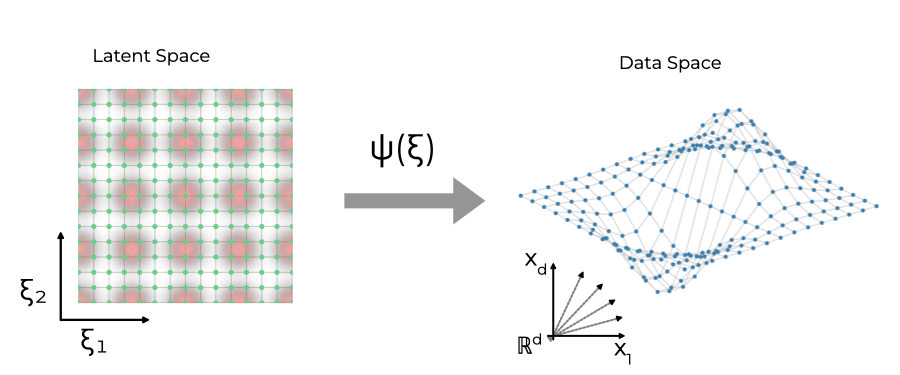
\includegraphics[width=\columnwidth]{robot-team-gtm/methods/gtm-diagram.png}
  \caption{Illustration of the GTM algorithm. On the left is a regular grid of
    $K$ many points (green) in the latent space represented by their coordinates
    $\xi_1$ and $\xi_2$. In red are the $M$-many radial basis functions which
    define the mapping $\psi$ from the latent space to the data space. Points in
    the latent space are mapped nonlinearly to the data space yielding an
    embedded manifold in $\mathcal{R}^d$, here shown in three dimensions.}
  \label{fig:gtm-diagram}
\end{figure}



Slices $R_{[:,n]}$ of the matrix $R$ define the responsibility of each latent node $\xi_k$ for the $n$th data record $\mathbf{x}_n$. Therefore, the final responsibility matrix after GTM training can be used to represent each record in the latent space by the following mean:
\begin{equation}\label{eq:mean-resp}
    \hat{\xi}_n = \sum_{k}^K R_{kn}\xi_k.
\end{equation}

A freely available implementation of the GTM algorithm was developed for this study and is accessible at \cite{gtm-code}. The code is written in the Julia programming language and complies with the Machine Learning in Julia (MLJ) common interface \cite{bezanson2012julia,blaom2020mlj}.

\subsection{UAV-Based Hyperspectral Imaging}

A Freefly Alta-X autonomous quadcopter was used as the UAV platform in this study. This UAV was equipped with a Resonon Pika XC2 visible+near-infrared (VNIR) hyperspectral imager to capture HSI with $462$ wavelengths per pixel ranging from $391$ to $1011$ nm. This imager is in a pushbroom configuration so that HSI are captured one scan-line at a time resulting in data cubes consisting of $1000$ scan-lines with $1600$ pixels each. Additionally, the camera includes an embedded GPS/INS unit to enable georectification of collected HSI. An upward-facing Ocean Optics UV-Vis NIR spectrometer with a cosine corrector was also included to provide measurements of the incident solar irradiance spectrum. The configuration of the UAV with the attached hyperspectral imager is shown in Figure~\ref{fig:drone}. Data collection and processing were controlled by an attached Intel NUC small-form-factor computer. A detailed description of the UAV platform can be found in \cite{robot-team-1}.

To account for the variability of incident light, raw HSI are converted to units of reflectance using the downwelling irradiance spectrum simultaneously captured with each HSI. With the hyperspectral imager oriented to nadir, the reflectance is given by
\begin{equation}\label{eq:reflectance}
    \rho(\lambda) = \pi L(\lambda)/E_d(\lambda)
\end{equation}
where $L$ is the spectral radiance, $E_d$ is the downwelling irradiance, and a factor of $\pi$ steradians results from assuming Lambertian (diffuse) upwelling radiance \cite{ruddick2019review}. HSI collection was performed near solar noon to maximize the amount of incident sunlight illuminating the water. For the site in North Texas, this corresponded to an average solar zenith angle of $54.9^\circ$ for 23 November 2020. During flights, the hyperspectral imager was oriented to nadir, resulting in HSI with negligible sunglint effects.


\begin{figure}[H]
  \centering
  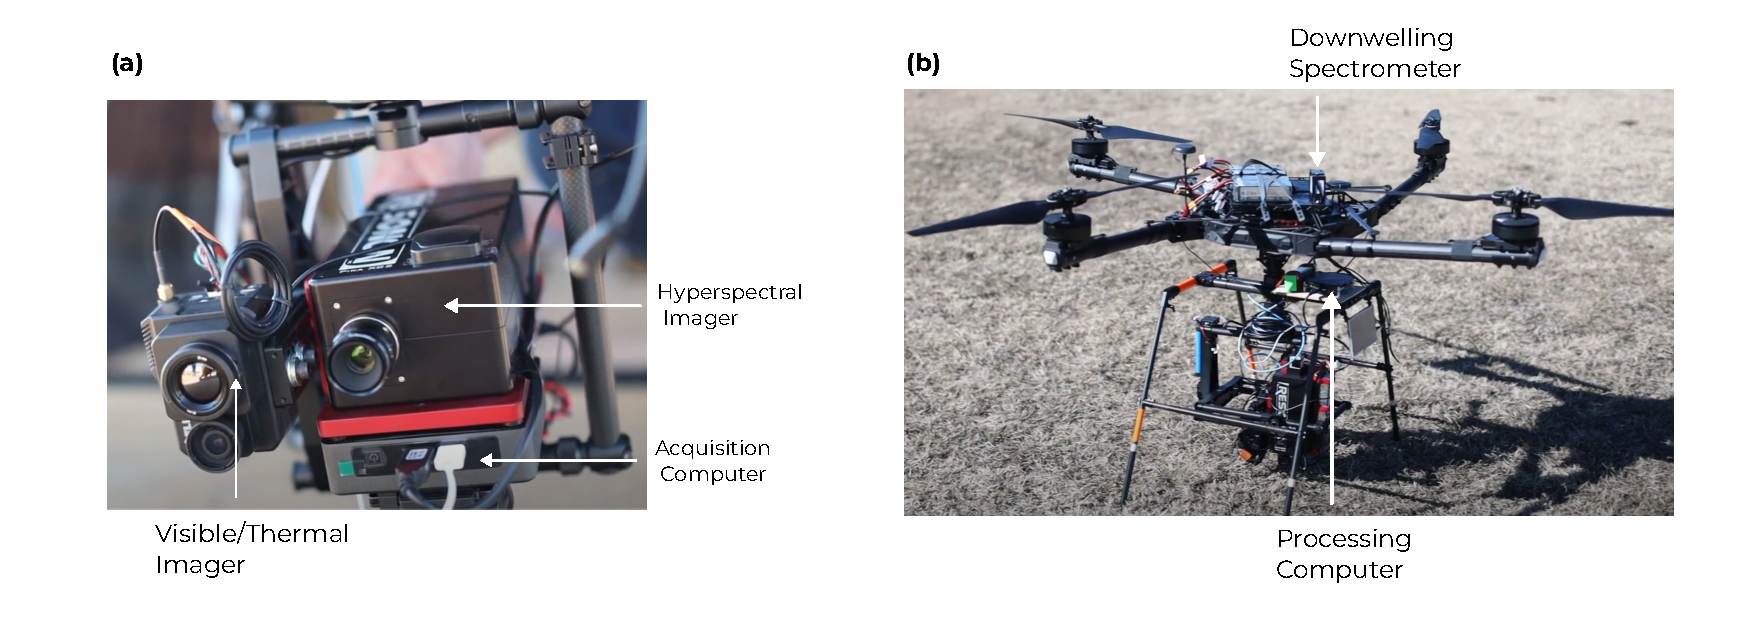
\includegraphics[width=\columnwidth]{robot-team-gtm/methods/annotated-drone.pdf}
  \caption{The UAV platform: (\textbf{a}) The Resonon Pika XC2 hyperspectral
    imager. (\textbf{b}) The Freefly Alta-X with the attached hyperspectral
    imager, processing computer, and downwelling irradiance
    spectrometer. \label{fig:drone}}
\end{figure}




After conversion to reflectance, each HSI must also be georectified to assign geographic coordinates to each pixel. The UAV flights were performed at an approximate altitude of $50$~m above the water so that the imaging surface can be considered to be flat. Consequently, HSI were rapidly georectified to a $10$ cm resolution using position and orientation data from the embedded GPS/INS, as outlined in refs. \cite{muller2002program, baumker2001new, mostafa2000multi}. An example hyperspectral data cube is illustrated in Figure~\ref{fig:sample-spectra}a  where the log10-reflectance values are plotted along the \emph{z}-axis for each pixel in the scene, and a psuedocolor image at the top of the data cube illustrates how the water would appear to the human eye from the perspective of the UAV.

As a final processing step before training each GTM, we limit the wavelengths of each HSI to $\lambda \leq 900$ nm, as wavelengths above $900$ nm showed significant noise. Additionally, each spectrum was rescaled to a peak value of $1.0$ to account for incident light variability between HSI.

\subsection{GTM Case Studies}\label{sec:case-studies}

To explore the ability of the GTM to segment HSI pixels and aid in source identification, we first consider a dataset of water-only spectra consisting of $>$36,000 records identified from collected HSI by a normalized difference water index (NDWI) greater than $0.25$, where the NDWI is defined as
\begin{equation}
    \text{NDWI} = \dfrac{\rho(550) - \rho(860)}{\rho(550) + \rho(860)}
\end{equation}
where $\lambda=550$ and $\lambda=860$ nm were chosen to represent the green and NIR bands as described in ref. \cite{ndwi}. We then apply the trained GTM to all water-only pixels to visualize the distribution learned by the GTM and examine spectra associated with a subset of nodes in the latent space in order to assess the small-scale spatial variability within the pond.

Next, we consider a dataset of combined HSI pixels including both water and land. To simulate the dispersion of a potential contaminant source, a rhodamine tracer dye was released into the western portion of the pond and two additional UAV flights were used to collect HSI capturing the evolution of the resulting plume. From these HSI, a collection of >145,000 pixels were sampled for model training. To demonstrate the ability to extract relevant spectral endmembers from the trained GTM, we utilize the exemplar spectra corresponding to open water, ground, nearshore algae, and rhodamine dye visually identified in Figure~\ref{fig:sample-spectra}. The responsibility matrix obtained by the trained GTM provides a probability distribution over the latent space nodes for every data record. We identify relevant endmembers for each reference spectrum via the set of nodes with nonzero responsibility. We then utilize the mapping $\psi$ to obtain the spectral representation of these nodes. Since the GTM is unsupervised, these extracted endmembers do not correspond to individual records but rather spectral features learned by the GTM. 

Values for the hyperparameters $m$, $s$, and $\alpha$ are determined by training multiple GTM models and selecting values which minimize the Bayesian Information Criterion (BIC) given by 
\begin{equation}
    \text{BIC} = P\ln(N) - 2\mathcal{L}
\end{equation}
where $P$ is the total number of model parameters, $N$ is the number of records in the dataset, and $\mathcal{L}$ is the log-likelihood defined in Equation~\eqref{eq:llh}.

The normalized spectral similarity score (NS3) introduced by Nidamanuri and Zbell combines the root mean square (RMS) difference together with the spectral angle to provide a spectral distance function \cite{nidamanuri2010normalized}. For two spectra $\rho_1(\lambda)$ and $\rho_2(\lambda)$, it is defined by
\begin{equation}
    \text{NS3}(\rho_1, \rho_2) = \sqrt{RMS(\rho_1, \rho_2)^2 + (1-\cos\theta)^2}
\end{equation}
where
\begin{align}
    \text{RMS}(\rho_1, \rho_2) &= \sqrt{\frac{1}{N-1}\sum_\lambda \left(\rho_{1}(\lambda) - \rho_2(\lambda) \right)^2} \\
    \cos\theta &= \frac{\langle \rho_1 , \rho_2 \rangle}{\lVert \rho_1\rVert \lVert \rho_2 \rVert}.
\end{align}

We use the NS3 together with extracted GTM endmembers to map the abundance of filamentous blue--green algae near the shore, as well as the evolution of the rhodamine dye plume. To do this, the GTM node with maximum responsibility is selected from the endmembers identified for the algae and rhodamine reference spectra. The distribution of NS3 values between each endmember and all HSI pixels is then used to select a suitable cutoff threshold. The area subsumed by HSI pixels with an NS3 below this threshold is then used to infer the spatial extent of algae and rhodamine in the pond. 




\section{Results}



\subsection{Water-Only Pixel Segmentation}


A GTM with $K=32\times 32$ nodes was trained on the dataset of water-only pixels described in Section ~\ref{sec:case-studies} in order to explore the distribution of reflectance spectra captured by the HSI. The resulting GTM is visualized in Figure~\ref{fig:gtm-water}. First, we note that the GTM has utilized most of the latent space as illustrated  Figure~\ref{fig:gtm-water}b where the position corresponding to the mean responsibility of each data point $\hat{\xi}_n$ has been plotted. For this water-only GTM, the spectra appear to be largely clustered toward the left edge, bottom, and right edge of the latent space. Spectral signatures corresponding to GTM nodes from the four corners and center of the latent space are shown in Figure~\ref{fig:gtm-water}c, illustrating the spectral variability represented across the latent space. 

\begin{figure}[H]
  \centering
  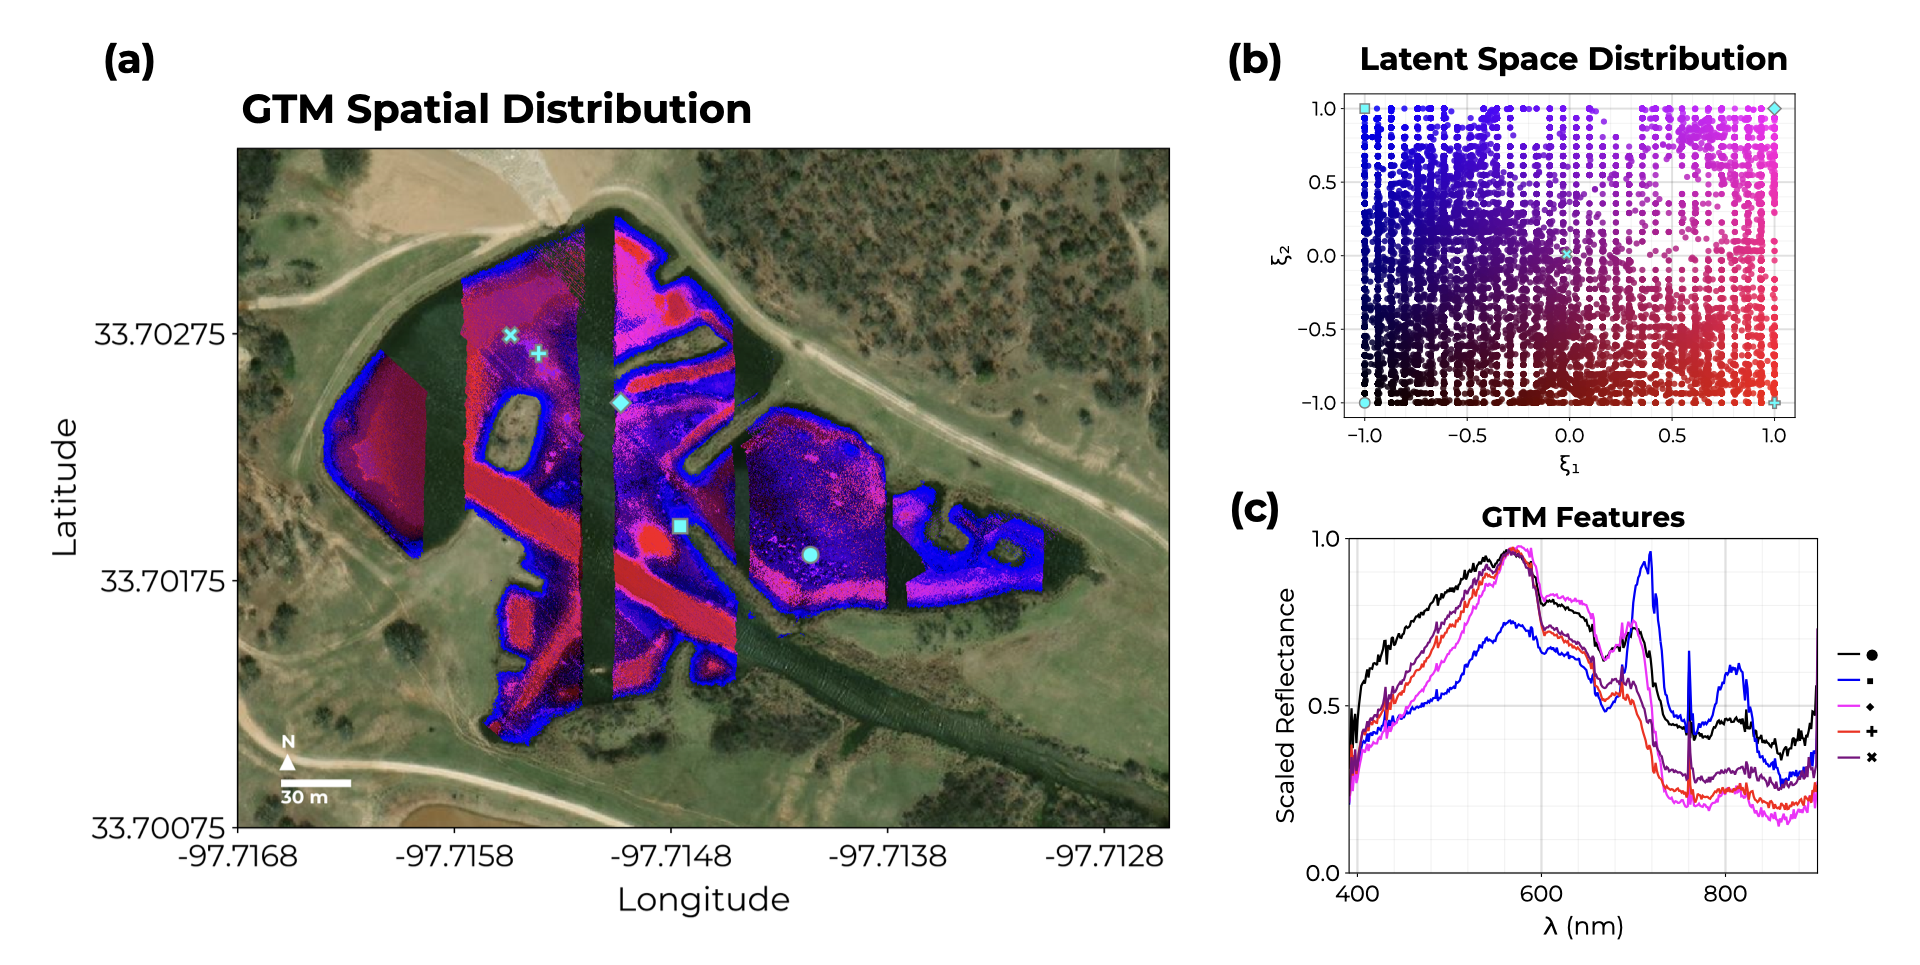
\includegraphics[width=\columnwidth]{robot-team-gtm/results/gtm-water.png}
  \caption{Visualization of the GTM trained solely on water pixels (no land and
    no rhodamine plume). Each data point is colored by computing the mean latent
    space position, $\hat{\xi}_n$ according to Equation~\eqref{eq:mean-resp}
    with red corresponding to the $\xi_1$ coordinate and blue corresponding to
    the $\xi_2$ coordinate. (\textbf{a}) Spatial distribution learned by the
    GTM. (\textbf{b}) The distribution of data in the latent space. Nodes
    corresponding to the four corners and center of the latent space are
    identified with cyan markers. (\textbf{c}) reflectance spectra corresponding
    to the selected GTM nodes computed via the nonlinear mapping
    $\psi(\xi_k$).}
  \label{fig:gtm-water}
\end{figure}

To visualize the distribution of HSI learned by the GTM, we can associate a color with each dimension of the latent space. In Figure~\ref{fig:gtm-water}, we used the red channel to represent $\xi_1$ and the blue channel to represent $\xi_2$. Applying the trained GTM to compute mean node responsibilities for all water pixels in collected HSI allows us to illustrate the spatial distribution of the spectra on a map, as shown in Figure~\ref{fig:gtm-water}c. Here, we observe a clear distinction between water near the shore and water in the middle of the pond. Additionally, the eastern alcove of the pond is significantly more blue than the rest of the water. We note that flow through this region is restricted by the small entrance near the cyan square shown in panel a. However, despite its similar depth and surface characteristics, the GTM distinguished this region from the rest of the water.

The close proximity of highly dissimilar GTM classes illustrated by sharp color gradients in the map reflects the small-scale spatial variability typical of inland water bodies like this pond. For example, water near the cyan diamond in panel a of Figure~\ref{fig:gtm-water} includes both blue and red pixels in close proximity. As shown in Figure~\ref{fig:gtm-water}b, these colors correspond to the top-left and bottom-right corners of the GTM latent space. As the GTM model maps neighboring nodes to similar spectra, this region includes maximally dissimilar pixels. Furthermore, this point is away from the shore where the depth is approximately uniform. The precision parameter $\beta$ learned by the GTM enables the model to account for spectral variability so that effects from localized disturbances such as surface ripples are constrained to small displacements in the latent space. With these considerations in mind, contrast in this region of the pond therefore reflects real variability of water composition, surface sediments, and vegetation.


\subsection{Endmember Extraction}

A second GTM was trained on the combined dataset of HSI with pixels covering shore, water, and the rhodamine tracer dye release. The resulting latent space distribution is shown in Figure~\ref{fig:gtm-ndvi}, where each sample is plotted at the position of the mean node responsibility and colored by the normalized difference vegetation index (NDVI) computed from the original reflectance spectrum. The NDVI is a spectral index sensitive to variations in vegetation health with negative values corresponding to water, small positive values corresponding to sparse vegetation, and large values near $1$ corresponding to dense vegetation \cite{thenkabail2018hyperspectral}. From this, we see that the GTM can clearly separate spectra by vegetation content with high values concentrated to the left of the latent space and negative, water-based pixels concentrated to the right. Additionally, the position of exemplar spectra for algae, rhodamine, water, and ground points are included as color-filled circles, further illustrating the separation of distinct sources obtained by the GTM. We note that a portion of the nearshore algae was observed to float at the surface of the water near the shore. Consequently, the position of the exemplar spectrum in Figure~\ref{fig:gtm-ndvi} used for algae occurs at a non-negative NDVI. The accumulation of records with negative NDVI values in close proximity (in the latent space) to the selected algae spectrum reflects the presence of algae within the water.


\begin{figure}[H]
  \vspace{-0.25cm}
  \centering
  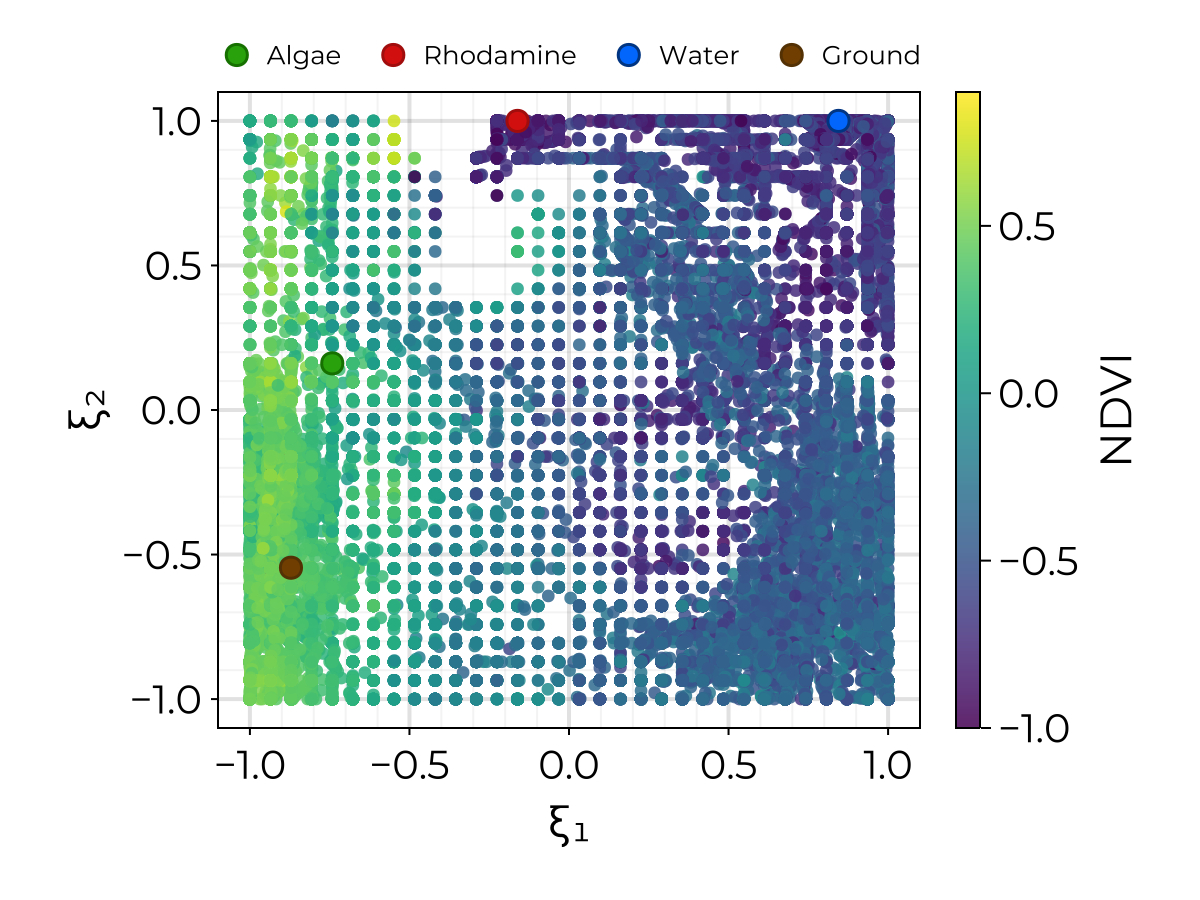
\includegraphics[width=0.7\columnwidth]{robot-team-gtm/results/square-ndvi.png}
  \vspace{-0.75cm}
  \caption{GTM latent space visualization: Each sample spectrum from the dataset
    of combined HSI covering shore, water, and the rhodamine dye release are
    plotted in the GTM latent space at the location of the mean node
    responsibility, $\hat{\xi}_n$. Points are colored according to the NDVI
    computed from the original reflectance spectra. The locations of exemplar
    spectra for algae, rhodamine, water, and ground points in the latent space
    are included as color-filled circles. Spectra from the shore and open water
    are clearly separated into different regions of the latent
    space.}
  \label{fig:gtm-ndvi}
\end{figure}



As outlined in Section~\ref{sec:gtm-overview}, there are three hyperparameters that need to be chosen to fit a GTM model: the number of RBF centers $M$ = m$^2$ with $m$ the number along each axis, the scale factor $s$ which controls the RBF overlap, and the regularization parameter $\alpha$. To choose appropriate values, we performed a grid search for $m$ values between $2$ and $20$, $s$ values between $0.1$ and $3.0$, and $\alpha$ values between $0.001$ and $10.0$. The best values were determined as those which minimized the BIC, with $m=14$, $s=1.0$, and $\alpha=0.1$, respectively. Heatmaps comparing the BIC for different hyperparameter values are provided in Figure~\ref{fig:hp-results}, and a table of the top 25 models is given in Table~\ref{tab:hp-search}.  Since the matrix of RBF activations $\Phi$ need only be computed once at the GTM initialization step, the number of latent nodes given by $K=k^2$ can be chosen to be large enough to ensure a smooth mapping. We found that a value of $k=32$ provided a sufficient number of GTM nodes without significantly impacting training time.

\begin{figure}[H]
  \centering
  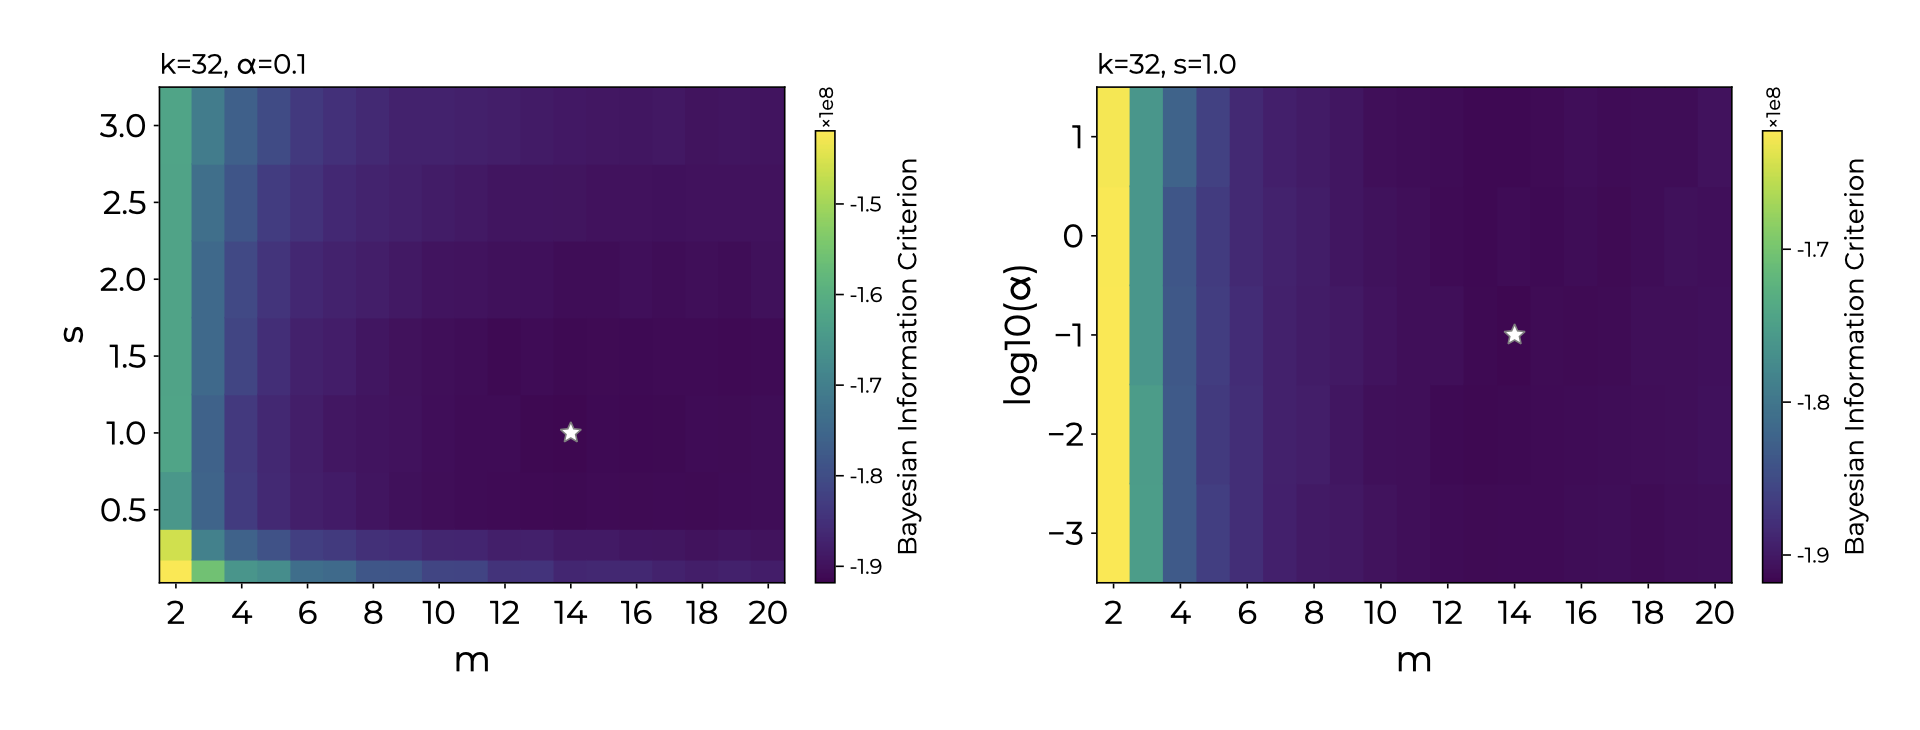
\includegraphics[width=\columnwidth]{robot-team-gtm/results/bic.png}
  \caption{Results of the hyperparameter search: (\textbf{left}) Variation in
    BIC with $m$ and $s$ for fixed $\alpha=0.1$. (\textbf{right}) Variation in
    BIC with with $m$ and $\alpha$ for fixed $s=1.0$. The white star in each
    plot indicates the parameters with the lowest BIC across the entire
    parameter search.}
  \label{fig:hp-results}
\end{figure}


\begin{table}
  \caption{The top 25 models from the hyperparameter search. A variety of GTM
    were trained to explore the the impact of varying m, $\alpha$, and s. The
    Bayesian Information Criterion (BIC) and Akaike Information Criterion (AIC)
    are given in the final two columns which can be used for hyperparameter
    selection.}
  \label{tab:hp-search}
  \begin{center}
  \begin{tabular}{cccccc} \hline
    \textbf{m} & \textbf{\boldmath$\alpha$} & \textbf{s} & \textbf{k} & \textbf{BIC} & \textbf{AIC} \\ \hline
    \textbf{14} & \textbf{0.1} & \textbf{1.0} & \textbf{32} & $\mathbf{-1.918 \times 10^8}$ & $\mathbf{-1.926 \times 10^8}$\\
    13 & 0.01 & 1.0 & 32 & $-1.917 \times 10^8$ & $-1.923 \times 10^8$\\
    16 & 0.01 & 1.5 & 32 & $-1.917 \times 10^8$ & $-1.926 \times 10^8$\\
    14 & 10.0 & 1.0 & 32 & $-1.917 \times 10^8$ & $-1.924 \times 10^8$\\
    16 & 0.001 & 1.5 & 32 & $-1.917 \times 10^8$ & $-1.926 \times 10^8$\\
    13 & 1.0 & 1.0 & 32 & $-1.917 \times 10^8$ & $-1.923 \times 10^8$\\
    13 & 10.0 & 1.0 & 32 & $-1.917 \times 10^8$ & $-1.923 \times 10^8$\\
    14 & 0.001 & 1.5 & 32 & $-1.916 \times 10^8$ & $-1.924 \times 10^8$\\
    13 & 0.1 & 1.0 & 32 & $-1.916 \times 10^8$ & $-1.923 \times 10^8$\\
    14 & 0.01 & 1.0 & 32 & $-1.916 \times 10^8$ & $-1.924 \times 10^8$\\
    15 & 0.01 & 1.5 & 32 & $-1.916 \times 10^8$ & $-1.925 \times 10^8$\\
  \end{tabular}
  \end{center}
\end{table}


Examining the latent space distribution learned by the GTM provides an unsupervised method to extract endmember spectra corresponding to unique sources within the imaging scene. To demonstrate this clearly, we consider the exemplar spectra visually identified in Figure~\ref{fig:sample-spectra}. Using the trained GTM, we can compute spectral signatures for each node in the latent space via the nonlinear mapping $\psi$. The responsibilities $R_{kn}$ therefore correspond to the contributions of the $kth$ node $\xi_k$ to the $n$th sample spectrum in the dataset. Endmembers are identified by nodes with nonzero responsibility values for each of the selected exemplar spectra and are plotted in Figure~\ref{fig:spectral-signatures}. We note that these extracted endmembers are able to accurately capture the shape of each exemplar spectrum including thin reflectance peaks. The GTM has also managed to smoothly interpolate through noisy wavelengths, as shown by the water and algae endmembers for $\lambda > 800$ nm. 

\clearpage
\newpage

\begin{figure}[H]
  \centering
  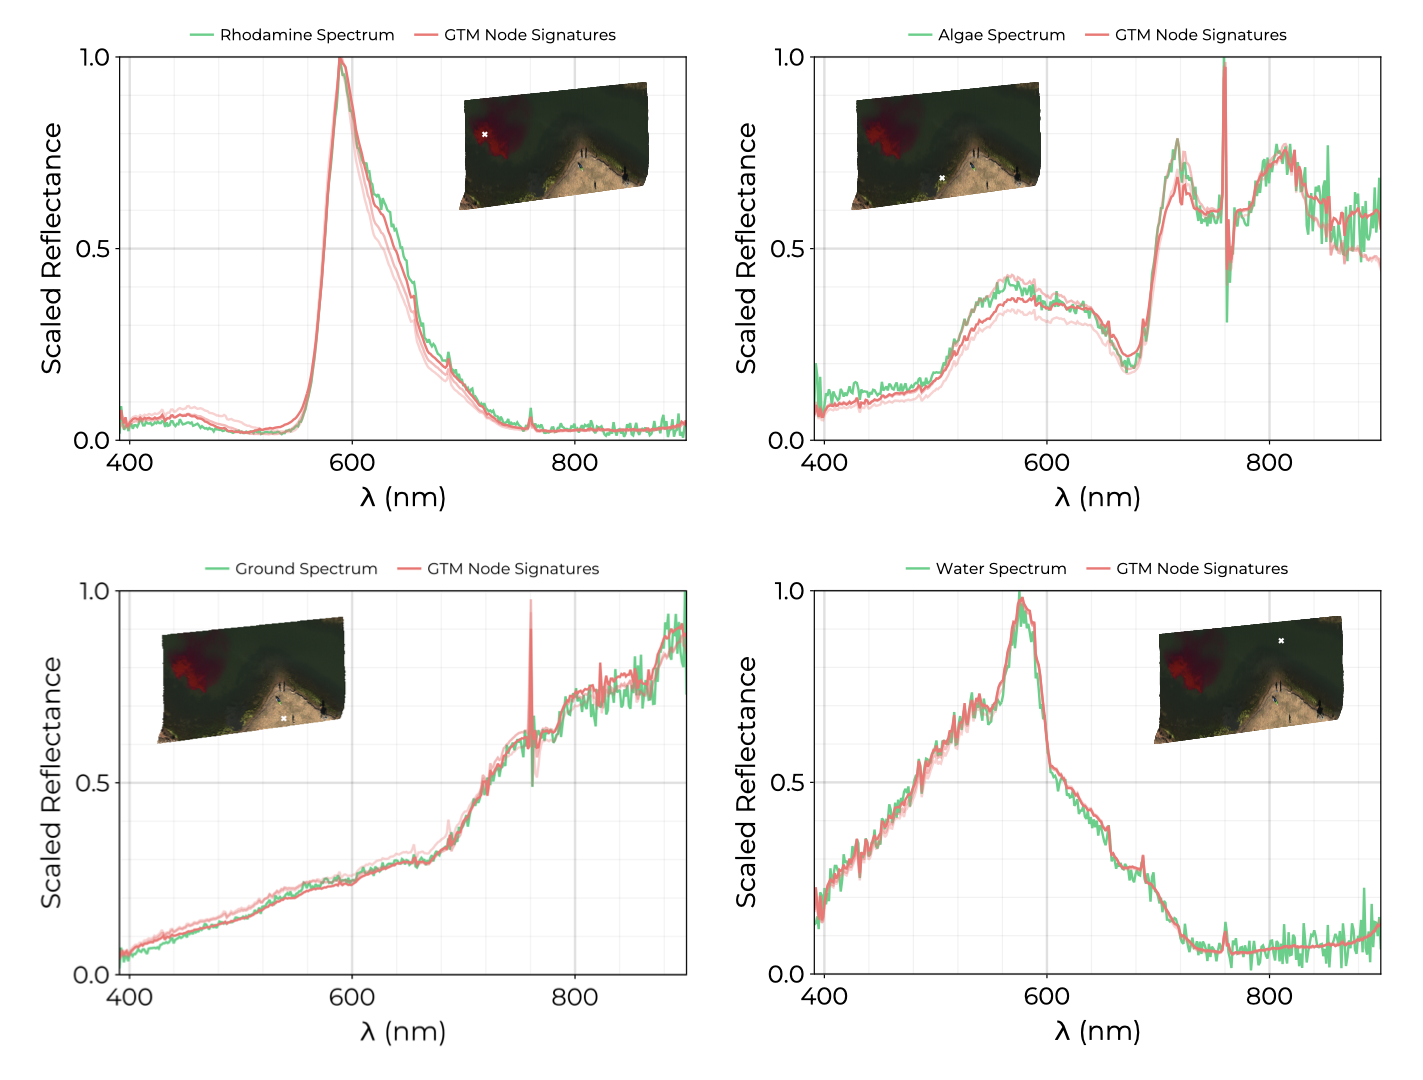
\includegraphics[width=\columnwidth]{robot-team-gtm/results/spectral-signatures.png}
  \caption{Spectral signatures $\psi(\xi_k)$ corresponding to GTM nodes with
    nonzero responsibility for the rhodamine dye plume (\textbf{top left}),
    nearshore algae (\textbf{top right}), ground (\textbf{bottom left}), and
    open water (\textbf{bottom right}). A pseudocolor image is inset into each
    plot with the location of the exemplar spectrum marked with a white
    circle.}
  \label{fig:spectral-signatures}
\end{figure}

\clearpage
\newpage

\subsection{Abundance Mapping with NS3}


Spectral endmembers extracted from the GTM can be used to map the abundance of water constituents in HSI by identifying pixels with a NS3 value below a given threshold. In Figure~\ref{fig:algae-map}, we demonstrate this by using the extracted algae endmember spectrum to map the abundance of filamentous blue--green algae near the western shore of the pond. The distribution of NS3 values was multimodal with a majority of pixels above $0.4$ belonging to dissimilar spectra. Consequently, a cutoff threshold of $0.4275$ was chosen to distinguish algae values corresponding to the $20$th-quantile of the NS3 distribution. The estimated area subsumed by algae is shown in Figure~\ref{fig:algae-map} and calculated to be $587.3$ m$^2$. Similarly, we are able to track the evolution of the rhodamine dye release into the western portion of the pond by computing the NS3 for HSI collected across multiple flights. Here, the same cutoff threshold was used corresponding to the $33$rd-quantile of the NS3 distribution. In the left panel of Figure~\ref{fig:rhodamine-map}, we see that the dye plume initially encompasses an area of roughly $330.7$~m$^2$. A second flight performed 15 min later reveals the dye plume to have increased to an area of $1495.6$ m$^2$. The increase in NS3 values between flights reflects the dilution of dye as it diffused into the water.

\clearpage
\newpage

\begin{figure}[H]
  \centering
  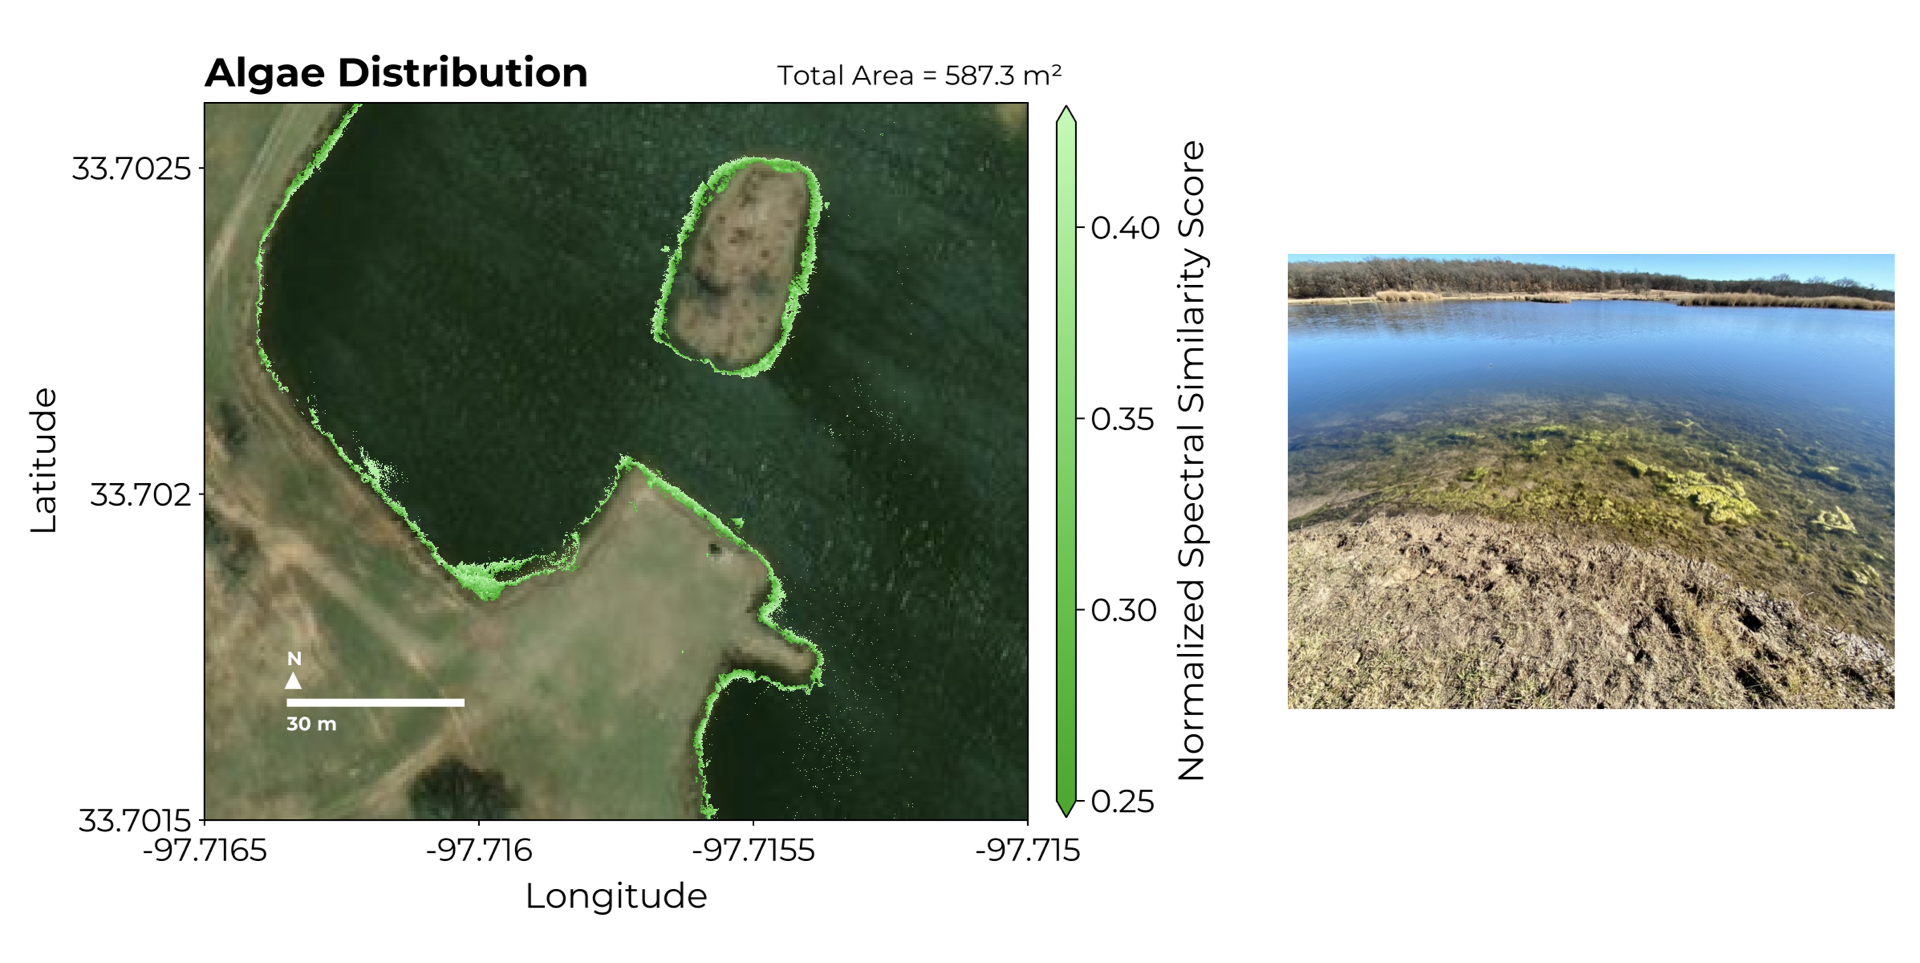
\includegraphics[width=\columnwidth]{robot-team-gtm/results/algae.png}
  \caption{Using the spectral endmember assigned to algae from the trained GTM
    together with the NS3, we are able to estimate the algal abundance near the
    shore. (\textbf{Left}) NS3 values of pixels below a threshold of 0.4275
    corresponding to a total area of $587.3$ $m^2$. (\textbf{Right}) A picture
    of the pond near the shore showing the algae.}
  \label{fig:algae-map}
\end{figure}


\begin{figure}[H]
  \vspace{-1cm}
  \centering
  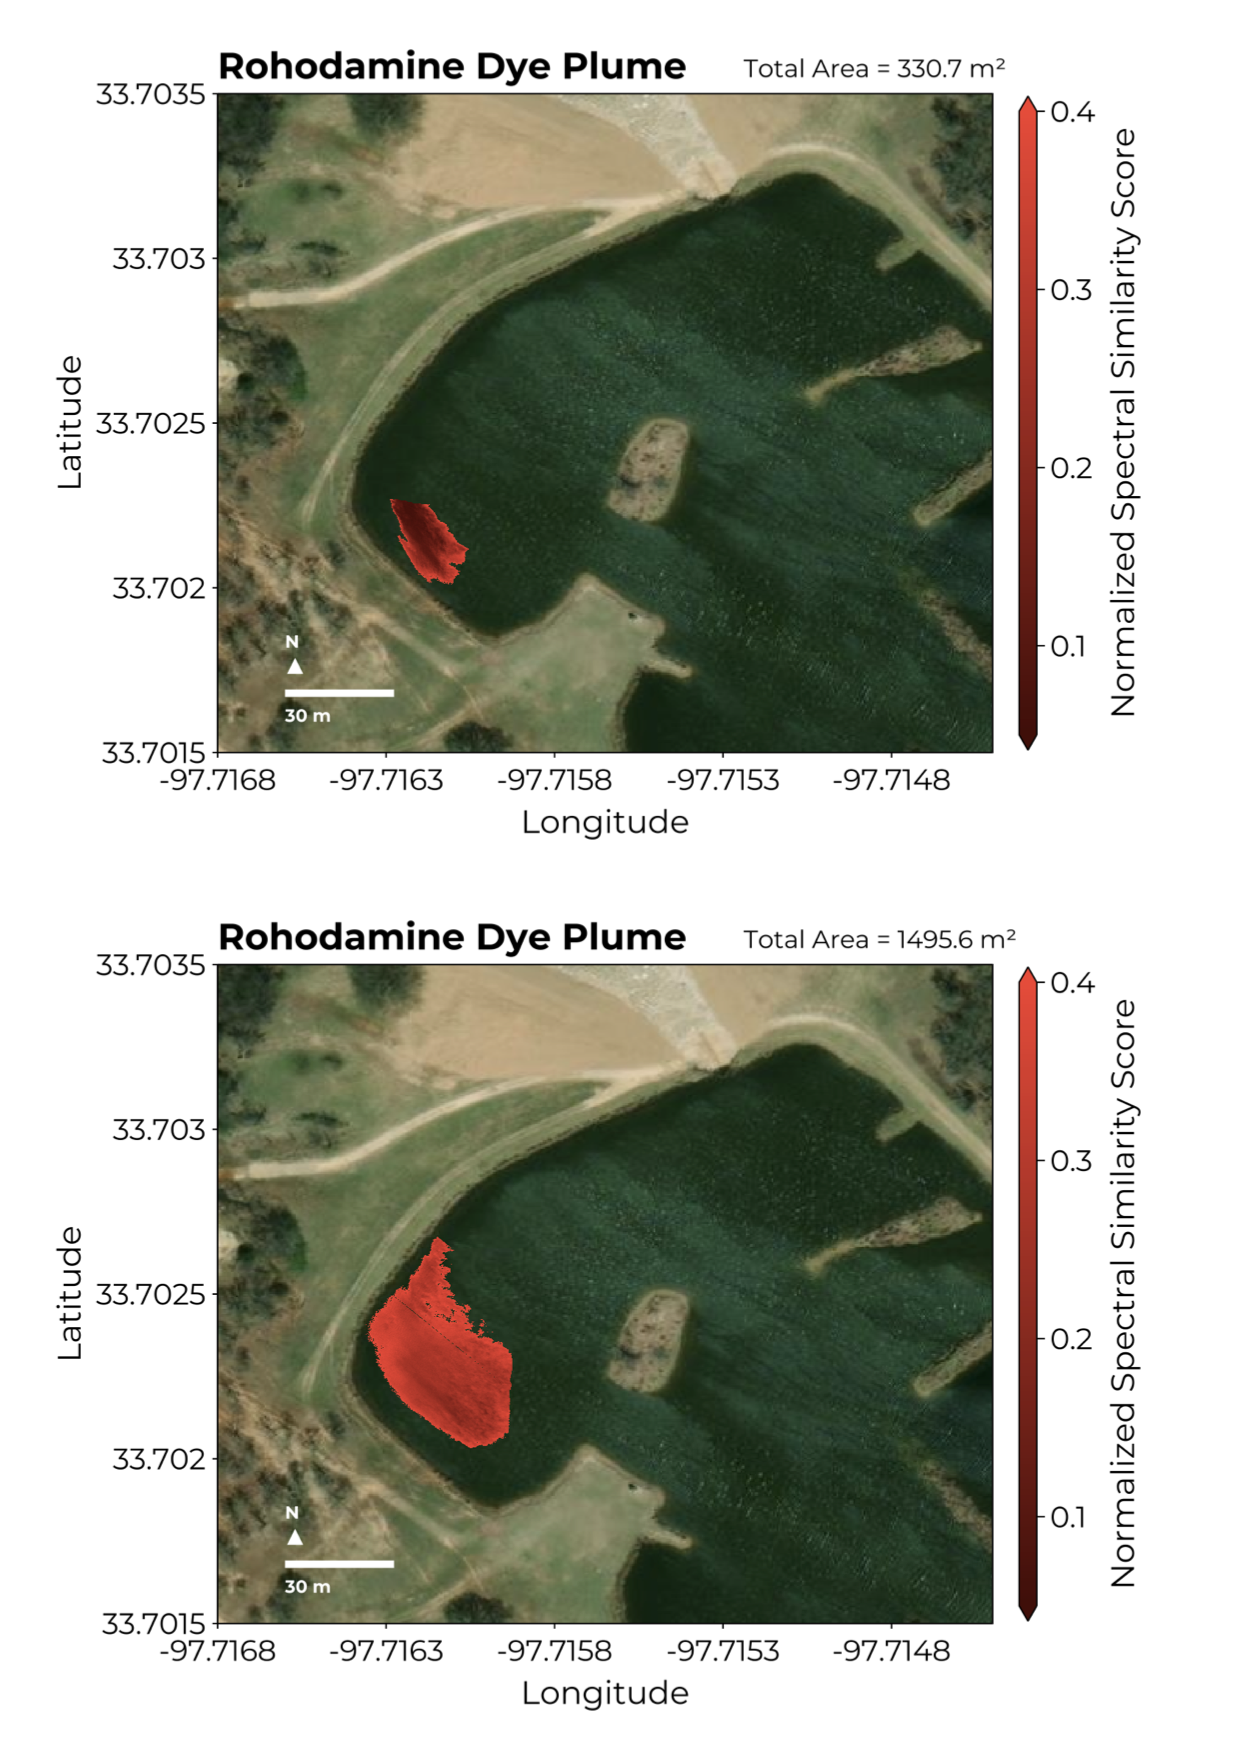
\includegraphics[width=0.85\columnwidth]{robot-team-gtm/results/rhodamine-vertical.png}
  \caption{Using the spectral endmember assigned to Rhodamine from the trained
    GTM together with the NS3, we are able to map the evolution of the dye plume
    across two UAV flights. (\textbf{top}) The initial dye plume corresponding
    to a total area of $330.7$ m$^2$. (\textbf{bottom}) The same dye plume
    imaged approximately 15 min later extends to a total area of $1495.6$
    m$^2$.}
  \label{fig:rhodamine-map}
\end{figure}

\clearpage
\newpage



\section{Discussion}

The application of UAV-based hyperspectral imaging (HSI) for water quality assessment is gaining significant traction due to its ability to efficiently capture detailed spectral data at high spatial resolutions. Most studies using UAVs have employed supervised techniques that map the captured spectra to specific water quality parameters of interest. For example, Lu et al. evaluated a variety of machine learning methods for the extraction of chlorophyll-a and suspended sediment concentrations from HSI using data from UAV flights over 33 sampling locations \cite{lu2021retrieval}. However, this approach relies on the collection of paired in situ data, which can be challenging to obtain in sufficient quantities to facilitate model training. Additionally, supervised methods require prior knowledge of expected sources in order to select and calibrate suitable reference instruments. Using models purpose-built for specific water quality parameters like chlorophyll-a or turbidity discards potential information contained in HSI, which can reveal unanticipated sources. Therefore, unsupervised methods which aid in the visualization of HSI and enable the identification of spectral endmembers within the imaging scene are needed to complement these supervised approaches.

Recently, some researchers have begun to explore endmember extraction using UAV-based imaging where the increased spatial resolution provided by UAV platforms is hypothesised to yield more pure pixels than their satellite counterparts. For instance, Alvarez et al. used multispectral UAV imagery to extract endmembers which were then applied to unmix remote sensing data for plant abundance estimation across a broad region of France~\cite{alvarez2020can}. Similarly, Gu et al. explored UAV-to-satellite hyperspectral unmixing by applying endmembers extracted from UAV-based HSI to satellite observations \cite{gu2023intrinsic}. These studies underscore the potential of combining endmember extraction techniques with UAV-based HSI, which has yet to see widespread adoption for water quality analysis.

In this study, we explored the GTM as a unsupervised approach to simultaneously enable visualization of HSI and perform endmember extraction of spectral signatures. First, we showed how the representation of data in the latent space of the GTM given by the mean responsibility can be used to visualize the small-scale structures within inland water bodies as evidenced in Figure~\ref{fig:gtm-water}. In particular, we note that the sharp gradients in colors found when visualizing the spatial distribution of GTM nodes across the pond reflects significant spectral variability at the submeter scale. % Please check intended meaning is retained.
This has important consequences for water quality assessment where the location of in situ data collection will have a strong impact on the ability of any model to predict water quality parameters from HSI. Visualizing the distribution of spectra from collected HSI is therefore highly relevant to guide in situ data collection, as shifting the sampling location by as little as a meter can lead to significant differences in measured values. 

Based on these observations, one clear application of the GTM for real-time
water quality assessment is for intelligently guided reference data collection.
In our previous work, we showed that coordinating UAV-based hyperspectral
imaging with in situ data collection by an autonomous boat can dramatically
improve the inversion of water quality parameters from HSI pixels
\cite{robot-team-2}. However, the spatial distributions of parameters such as
chlorophyll-a, blue--green algae, and temperature are often highly dissimilar
posing a challenge for optimal route planning. Since  GTM estimates the full
distribution of reflectance spectra and not a single water quality parameter,
one could construct a prize collecting travelling salesman problem (PC-TSP)
which seeks to find the optimal route maximizing the area explored in the GTM
latent space \cite{balas2007prize}. Similar approaches have been used to guide
data collection with autonomous vehicles to optimize data quality subject to
resource constraints \cite{suryan2020learning}.

The second application of the GTM presented in this study is for the
unsupervised extraction of endmembers corresponding to unique sources observed
in the HSI. Here, the GTM is an attractive choice, as it does not rely on the
assumptions of linear mixing and the presence of pure pixels which are easily
broken by the effects of multiple scattering in realistic scenarios
\cite{nonlinearity-in-hsi}. Additionally, because the GTM is a probabilistic
model, the values of model hyperparameters can be selected objectively using
information criteria like the BIC. This is a clear advantage over similar
methods like the SOM, on which the GTM is based. Endmembers identified for
exemplar spectra corresponding to rhodamine, algae, ground, and water pixels
demonstrate that the method can successfully identify spectral signatures
corresponding to diverse sources. If a set of labeled spectra for known sources
are available, their representation in the GTM latent space could be used to
perform a semisupervised classification, similar to the SOM approach developed
by Riese et al. \cite{riese2019supervised}. For example, in clear waters where
variation in sediments and vegetation at the pond floor will contribute to
observed spectral variability, the distribution learned by the GTM can be paired
with in situ data to classify the surface type.


% something about abundance mapping
Once endmembers are identified, estimating their abundance using the NS3
provides a quick method to map the distribution of sources in water. We note
that the spatial distribution of algae mapped in Figure~\ref{fig:algae-map}
realistically reflects clustering of algae near the shore. Additionally, the
ability for the UAV to quickly survey the same area in rapid succession is
highly advantageous for tracking the diffusion of point sources, as demonstrated
in Figure~\ref{fig:rhodamine-map} for the rhodmaine dye release.

The primary limitation of the GTM is that the number of nodes increases
exponentially with the dimension of the latent space. However, when constrained
to two dimensions, in order to enable visualization of the resulting map, the
number of latent nodes has a negligible impact compared with the size of the
dataset on which it is trained. Additionally, the GTM considers individual HSI
pixels and does not exploit spatial structure like other methods, such as
convolutional autoencoders and non-negative matrix factorization using
superpixels \cite{palsson2020convolutional,unmixing-nmf-review}. Extensions
to  GTM have been proposed to enable batch training for large datasets, as well
as manifold-aligned noise models which replace the fixed precision parameter
$\beta$ with a full covariance matrix \cite{gtm-developments}.

\textcolor{red}{Add an additional note about updating the GTM to utilize
  adaptive mixing coefficients $\pi_k$ as suggested in \cite{gtm-orig, gtm-developments}.}

Finally, we note that the representation obtained by  GTM can be used for
nonlinear feature extraction to improve supervised models. Traditionally, PCA is
used as a common preprocessing technique to reduce high-dimensional HSI by
keeping the first $r$-many principal components. For example, Uddin et al.
report improved classification of HSI by using PCA to extract features for a
support vector machine \cite{uddin2021pca}.  GTM can similarly be used to
provide a sparse representation of the input data via the latent node
responsibilities $R_{kn}$ obtained for each record.

